%   % !TEX root = ../../VIII,3_Rahmen-TeX_8-1.tex
%  
%   Band VIII, 3		Rubrik STOSS
%
%   Signatur/Tex-Datei:	LH_37_05_024
%
%   RK-Nr. 	60282		\ref{RK60282}
%
%   Überschrift: 	De legibus concursus
%   
%   Unterrubrik:			DCC plus ?
%
%   Datierung:		Winter 1676/1677 (?) bis Januar 1678
%
%   edlabels:			0
%
%   Diagramme: 		1
%
%
%   NB: 						(Anmerkungen)					??
%
%
%
\selectlanguage{ngerman}
\frenchspacing
%
\begin{ledgroupsized}[r]{120mm}
\footnotesize
\pstart
\noindent\textbf{Überlieferung:}
\pend
\end{ledgroupsized}
%
\begin{ledgroupsized}[r]{114mm}
\footnotesize
\pstart \parindent -6mm
\makebox[6mm][l]{\textit{L}}%
Aufzeichnung:
LH~XXXVII~5 Bl.~24. 
Ein Blatt~8\textsuperscript{o},
am Rand tlw. beschnitten;
Papiererhaltungsmaßnahmen.
Zwei Seiten.
\pend
\end{ledgroupsized}
%
%
\vspace{5mm}
\begin{ledgroup}
\footnotesize
\pstart
\noindent%
\textbf{Datierungsgründe:}%
\label{LH_37_05_024_Datierung}
Gegenstand der Aufzeichnung N.~\ref{RK60282} %??S03 
\textit{De legibus concursus} \textendash\ kaum mehr als eine Notiz, die skizzenhafte Gedanken festhält \textendash\ ist die Kinematik des gemeinsamen Schwerpunkts zweier Körper, die sich in einem Fluidum aneinander bewegen und gegebenenfalls aufeinander stoßen.
Der Titel zeigt, dass die Stoßlehre Ausgangspunkt der Fragestellung ist.
Dies rückt N.~\ref{RK60282} %??S03 
inhaltlich in die Nähe weiterer in diesem Band edierter Texte, in denen Leibniz im Rahmen seiner Untersuchung über die Stoßgesetze Gedankenexperimente entwirft, um das Gesetz der gleichförmigen Bewegung des gemeinsamen Schwerpunkts nachzuweisen:
In den Entwürfen N.~\ref{RK57266-1} %?? Elastrum est causa imperfectionis, 
(S.~\refpassage{LH_37_05_162r_Gedankenexperiment-1}{LH_37_05_162r_Gedankenexperiment-2}) und N.~\ref{RK57268} %?? Specimina artis condendi theoremata
(Randbemerkung zu S.~\refpassage{37_05_144r-145v_12a}{37_05_144r-145v_12b}), welche eigenhändig auf März bzw. Mai 1677 datiert sind,
liegen klare aber knappe Andeutungen auf diese Thematik vor, wohingegen die im Januar 1678 verfasste \textit{Scheda IX de corporum concursu} eine ausführliche Beschreibung ausgeklügelter Gedankenexperimente liefert (N.~\ref{dcc_09}, %??S01\textsubscript{11}, 
S.~\refpassage{LH_37_05_088rv_cntrmgrvtts-1}{LH_37_05_088rv_cntrmgrvtts-2}).
Die inhaltliche Verwandtschaft mit diesen Texten legt nahe, auch für N.~\ref{RK60282} %??S03 
eine Entstehungszeit zwischen Frühjahr 1677 und spätestens Januar 1678 anzunehmen.
\pend%
%
\pstart%
Da Leibniz seit seiner Beschäftigung mit Huygens' Stoßlehre im Sommer 1669 das Gesetz der gleichförmigen Bewegung des Schwerpunkts kannte (vgl. \textit{LSB} VI,~2 N.~38,\cite{02025} S.~158.1\textendash8, 159.3\textendash7), ist eine auch erheblich frühere Datierung der Aufzeichnung N.~\ref{RK60282} %??S03 
% \textendash\ etwa auf die Pariser Zeit \textendash\ 
grundsätzlich möglich.
Sie erweist sich aber als unwahrscheinlich, weil Leibniz nach heutigem Wissensstand die Kinematik des gemeinsamen Schwerpunkts aufeinander stoßender Körper erstmals in den genannten Texten N.~\ref{RK57266-1} %?? Elastrum est causa imperfectionis 
und N.~\ref{RK57268} %?? Specimina artis condendi theoremata
als Frage thematisiert und vornehmlich in den \textit{Schedae de corporum concursu} behandelt (zunächst in N.~\ref{dcc_02-1} %??S01\textsubscript{2} 
bis N.~\ref{dcc_03}). %??S01\textsubscript{4} 
Allerdings fehlt in N.~\ref{RK60282} %??S03 
\textendash\ anders als % in N.~\ref{RK57266-1}?? %?? Elastrum est causa imperfectionis, 
% und 
in den übrigen genannten Texten aus dem Zeitraum von März 1677 bis Januar 1678 \textendash\ 
der grundlegende Hinweis darauf, dass mit den entworfenen Gedankenexperimenten das Gesetz der gleichförmigen Bewegung des Schwerpunks nur dann nachgewiesen werden könne, wenn zusätzlich die Unmöglichkeit eines \textit{motus perpetuus artificialis} (und somit letztlich die notwendige Äquipollenz von Ursache und Wirkung) vorausgesetzt werde.
Dieser bemerkenswerte Tatbestand könnte als Zeichen dafür gedeutet werden, dass N.~\ref{RK60282} %??S03 
eher im Vorfeld des Entwurfs N.~\ref{RK57266-1} %?? Elastrum est causa imperfectionis 
entstand, d.h. noch im Winter 1676\textendash1677.
Aus demselben Grund kommt eine Datierung der vorliegenden Aufzeichnung % \textit{De legibus concursus} 
auf die Zeit nach N.~\ref{dcc_09} %??S01\textsubscript{11}, 
nicht in Frage.
Vielmehr dürfte N.~\ref{RK60282} %??S03 
noch vor Ende 1677 entstanden sein.%
\pend%
\end{ledgroup}%
%
%
\selectlanguage{latin}%
\frenchspacing%
%\newpage%
 \vspace{8mm}%
 \count\Bfootins=1000%
\count\Afootins=1200%
\count\Cfootins=1000
\pstart%
\normalsize%
\noindent%
%
\lbrack24~r\textsuperscript{o}\rbrack\ %%%% Blatt 24r
\hspace{39mm}
De legibus concursus%
\protect\index{Sachverzeichnis}{leges concursus}%
\protect\index{Sachverzeichnis}{concursus corporum}
\pend
\vspace{0.5em}%
%\vspace{\baselineskip}
%
\pstart%
\noindent%
Demonstrandum
%
\edtext{est primum}{%
\lemma{est}\Bfootnote{%
\textit{(1)}~in prim
\textit{(2)}~primum%
~\textit{L}}}
%
accuratissime,
quod duorum corporum
sive ascendentium%
\protect\index{Sachverzeichnis}{corpus ascendens}
sive descendentium%
\protect\index{Sachverzeichnis}{corpus descendens}
%
\edtext{sive concurrant sive non,}{%
\lemma{sive}\Bfootnote{%
\textit{(1)}~ante concursum sive post concursum
\textit{(2)}~concurrant sive non,%
~\textit{L}}}
%
\edtext{semper centrum gravitatis%
\protect\index{Sachverzeichnis}{centrum gravitatis}%
}{%
\lemma{semper}\Bfootnote{%
\textit{(1)}~in eadem recta
\textit{(2)}~centrum gravitatis%
~\textit{L}}}
%
eadem celeritate ascendat vel descendat.%
\protect\index{Sachverzeichnis}{celeritas ascensus}%
\protect\index{Sachverzeichnis}{celeritas descensus}
Quoniam nimirum gravitas totius%
\protect\index{Sachverzeichnis}{gravitas totius}
semper eadem
%
\edtext{est,
posito quod non impediatur.}{%
\lemma{est,}\Bfootnote{%
\textit{(1)}~nec a quoquam impeditur.
\textit{(2)}~posito quod non impediatur.%
~\textit{L}}}
%
\edtext{Sed jam}{%
\lemma{sed}\Bfootnote{%
\textit{(1)}~quoniam
\textit{(2)}~jam%
~\textit{L}}}
%
video ob accelerationem%
\protect\index{Sachverzeichnis}{acceleratio}
%
\edtext{et retardationem%
\protect\index{Sachverzeichnis}{retardatio}%
}{%
\lemma{et}\Bfootnote{%
\hspace{-0,5mm}retardationem
\textit{erg.~L}}}
%
continue augeri vel minui,
id ergo in calculum venire debet.%
\protect\index{Sachverzeichnis}{calculus}
%
\edtext{Notandum tamen etiam cum}{%
\lemma{Notandum}\Bfootnote{%
\hspace{-0,5mm}tamen
\textit{(1)}~cum
\textit{(2)}~etiam cum%
~\textit{L}}}
%
impeditur,
tamen in eadem semper linea 
%
\edtext{ferri centrum gravitatis,%
\protect\index{Sachverzeichnis}{centrum gravitatis}%
}{%
\lemma{ferri}\Bfootnote{%
\textit{(1)}~grave
\textit{(2)}~centrum gravitatis,%
~\textit{L}}}
%
etsi non semper ad easdem partes,
cum nimirum partes diversimode.
Cum autem non 
%
\edtext{impeditur,
ut autem}{%
\lemma{impeditur}\Bfootnote{%
\textit{(1)}~quod fit in
\textit{(2)}~ut autem in%
~\textit{L}}}
%
in eadem pergat linea
necesse est
in plano horizontali%
\protect\index{Sachverzeichnis}{planum horizontale}
eadem ferri celeritate.%
\protect\index{Sachverzeichnis}{celeritas centri gravitatis}
%
\lbrack24~v\textsuperscript{o}\rbrack\ %%%% Blatt 24v
%
\pend%
\pstart%
%\noindent%
Cogitandum etiam nullam amplius fore accelerationem%
\protect\index{Sachverzeichnis}{acceleratio}
cum sufficiens est liquidi ambientis resistentia.%
\protect\index{Sachverzeichnis}{resistentia liquidi ambientis}%
\protect\index{Sachverzeichnis}{liquidum ambiens}
Itaque hoc casu necesse est,%
\protect\index{Sachverzeichnis}{casus}
eadem celeritate ascendere%
\protect\index{Sachverzeichnis}{celeritas ascensus}
%
\edtext{et descendere.%
\protect\index{Sachverzeichnis}{celeritas descensus}%
}{%
\lemma{et}\Bfootnote{%
\hspace{-0,5mm}descendere
\textit{erg.~L}}}
%
%\pend 
%%
%\pstart 
%
Ex his Mechanicis%
\protect\index{Sachverzeichnis}{mechanica}
postea physica%
\protect\index{Sachverzeichnis}{physica}
concludi possunt,
nimirum necessario corpora
%
\edtext{gravia dura%
\protect\index{Sachverzeichnis}{corpus grave}%
\protect\index{Sachverzeichnis}{corpus durum}
esse Elastica.%
\protect\index{Sachverzeichnis}{corpus elasticum}%
}{%
\lemma{gravia}\Bfootnote{%
\textit{(1)}~esse Elastica.
\textit{(2)}~dura esse Elastica.%
~\textit{L}}}
%
\pend
%
\pstart%
Hinc jam facilis transitus ad eum casum
quo inclinatio plani%
\protect\index{Sachverzeichnis}{inclinatio plani infinite parva}
est infinite parva,
eo autem casu%
\protect\index{Sachverzeichnis}{casus}
manifestum est
nihil referre utcunque mutetur liquidum%
\protect\index{Sachverzeichnis}{liquidum ambiens}%
\lbrack,\rbrack\
semper enim aeque non resistit gravitati%
\protect\index{Sachverzeichnis}{gravitas}%
\lbrack;\rbrack\
vel potius fingamus corporum%
\protect\index{Sachverzeichnis}{corpus grave}%
\protect\index{Sachverzeichnis}{corpus leve}
%
\edtext{gravium vel levium}{%
\lemma{gravium}\Bfootnote{%
\hspace{-0,5mm}vel levium
\textit{erg.~L}}}
%
unum ascendere alterum descendere\lbrack,\rbrack\
neque ullam esse accelerationem
aut certe accelerationem%
\protect\index{Sachverzeichnis}{acceleratio}
tam esse parvam
ut haberi queat pro nulla,
respectu exigui spatii
quod percurritur,
et ob inclinationem exiguam%
\protect\index{Sachverzeichnis}{inclinatio plani infinite parva}
perinde erit ac si ponamus centrum gravitatis%
\protect\index{Sachverzeichnis}{centrum gravitatis}
aeque celeriter procedere.%
\protect\index{Sachverzeichnis}{processus centri gravitatis}%
\pend%
%
\vspace{1.5em} %%%%%%%%% Diagramm 1
\centerline{%
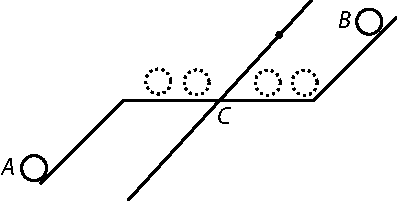
\includegraphics[width=0.42\textwidth]{%
gesamttex/edit_VIII,3/images/LH_37_05_024_d_024v.pdf%
}}
\vspace{0.0em}
\centerline{%
\lbrack\textit{Fig.~1}\rbrack%
}
%
\count\Bfootins=1200%
\count\Afootins=1200%
\count\Cfootins=1200
%
%
%%%% Ende des textes auf Bl. 24v
%